\chapter{几何、信息与黑洞面积定律}

\lectureoverview{所宣布的目的地是宇宙学，但通往它的最短道路始于回到狭义相对论。度规告诉我们时空的几何，而固有时为零的条件告诉我们光如何运动。我们将把这一条规则带入施瓦西几何，把视界与奇点区分开来，然后追问当黑洞辐射殆尽时信息会变成什么。答案始于普通的熵，终于贝肯斯坦的一比特论证：黑洞以视界面积而非体积为单位存储信息。}

苏斯金德暂时推迟了所承诺的对弦理论成败的清算。他说，时间已晚，实质内容比审计更有用。今晚的实质内容，是表述黑洞信息问题所需的最低限度的几何与热力学。

\section{关于光的一条规则}

狭义相对论把空间和时间当作一个几何对象。对于由\(dt,dx,dy,dz\)分隔的相邻事件，苏斯金德采用mostly-minus约定并写出
\begin{equation}
d\tau^2=dt^2-\frac{1}{c^2}\left(dx^2+dy^2+dz^2\right).
\end{equation}
时间部分与空间部分符号相反，这使闵可夫斯基几何区别于四维欧几里得几何。因子\(1/c^2\)只是协调单位；通过以相容的方式测量时间和距离，我们可以令\(c=1\)。

对于类时间隔\(d\tau^2>0\)，而\(d\tau\)是沿轨迹运动的时钟所记录的固有时。类空间隔则满足\(d\tau^2<0\)。今晚所需的情形恰好介于两者之间。光线沿\emph{零}轨迹运动，
\begin{equation}
d\tau^2=0.
\end{equation}
先限制为沿\(x\)轴的运动，得到
\begin{align}
0&=dt^2-\frac{dx^2}{c^2},\\
c\,dt&=\pm dx,\\
\frac{dx}{dt}&=\pm c.
\end{align}
这些符号描述向右和向左运动的光线。赋予\(c\)的数值在厘米被米或千米取代时会改变；不变的说法不是一个数，而是零条件。

广义相对论使度规复杂化，而不是使这条规则复杂化。以坐标\(x^\mu\)、\(\mu=0,1,2,3\)表示，
\begin{equation}
ds^2=g_{\mu\nu}(x)\,dx^\mu dx^\nu,
\end{equation}
其中重复指标求和，系数可以逐点变化。要找出局部允许的光的方向，令这个二次型为零。

\section{球坐标与施瓦西度规}

不旋转的黑洞是球对称的，因此笛卡尔坐标掩盖了有用的结构。令\(r\)度量径向距离，令\(\theta,\phi\)确定单位球面上的方向。其线元为
\begin{equation}
d\Omega^2=d\theta^2+\sin^2\theta\,d\phi^2.
\end{equation}
因此在半径为\(r\)的球面上，角位移贡献\(r^2d\Omega^2\)。球坐标下的平直时空为
\begin{equation}
d\tau^2=dt^2-\left(dr^2+r^2d\Omega^2\right),
\qquad (c=1).
\end{equation}

苏斯金德没有从爱因斯坦方程推导黑洞解。他把它写下来，并要求我们审视它。黑板明确地作出了预期的比较。

\begin{figure}[htbp]
\centering
\includegraphics[width=0.86\textwidth]{lecture_02_figure_02.png}
\caption{施瓦西形变之上的平直球面时空。重复出现的因子\(1-2GM/(c^2r)=1-R_s/r\)与径向草图同时可见。}
\lectureframe{00:19:12.520}
\end{figure}

对于质量为\(M\)的黑洞，定义施瓦西半径
\begin{equation}
R_s=\frac{2GM}{c^2}.
\end{equation}
外部线元为
\begin{equation}
d\tau^2=\left(1-\frac{R_s}{r}\right)dt^2
-\frac{dr^2/c^2}{1-R_s/r}
-\frac{r^2}{c^2}d\Omega^2.
\label{eq:schwarzschild-explicit-c}
\end{equation}
等价地，在令\(c=1\)之后，
\begin{equation}
ds^2=\left(1-\frac{2GM}{r}\right)dt^2
-\frac{dr^2}{1-2GM/r}-r^2d\Omega^2.
\label{eq:schwarzschild}
\end{equation}
在远处，\(R_s/r\ll1\)，平直球面度规回归。这个渐近检验比记住公式更重要，尽管苏斯金德推荐后者作为鸡尾酒会上的谈资。

\editorialnote{黑板在\(d\tau^2\)与\(ds^2\)之间交替，并且没有一致地显示每一个\(c\)因子。方程~\eqref{eq:schwarzschild-explicit-c}遵循讲座的时间坐标约定，其中\(t\)具有时间的量纲。带有\(x^0=ct\)的标准形式在代数上等价。}

\subsection{视界不是奇点}

在坐标中有两个半径看起来可疑。在自然单位下的\(r=R_s=2GM\)处，\(dt^2\)的系数为零，而\(dr^2\)的系数发散。在\(r=0\)处，曲率本身变为奇异。这些不是同一事件的两种版本：
\begin{equation}
\begin{aligned}
r=R_s &:\quad \text{horizon},\\
r=0 &:\quad \text{curvature singularity}.
\end{aligned}
\end{equation}

潮汐力给出了物理上的区分。引力场在延展物体上逐点变化：脚受到的拉力可能比头更强，拉伸身体，而横向方向被挤压。在视界处，这些潮汐力是有限的，而在质量足够大的黑洞的视界处，它们可以非常小。那里不必发生任何局部灾难性的事情。相反，在\(r=0\)处，潮汐力发散。\(r=R_s\)处令人警觉的系数标志着施瓦西坐标的缺陷；\(r=0\)处的奇点是物理的。

\editorialnote{曲率在\(r=R_s\)处的有限性可由Kretschmann标量\(R_{\mu\nu\rho\sigma}R^{\mu\nu\rho\sigma}=48G^2M^2/(c^4r^6)\)来检验，该标量在视界处有限，仅在\(r\to0\)时发散。这一不变量在讲座中并未写出，但它使潮汐力的区分变得精确。}

\section{视界附近的径向光}

现在回到那条规则。径向光线保持其角位置固定，因此\(d\Omega=0\)，而光线满足\(ds^2=0\)。在\(c=1\)单位下，方程~\eqref{eq:schwarzschild}给出
\begin{equation}
0=\left(1-\frac{2GM}{r}\right)dt^2
-\frac{dr^2}{1-2GM/r}.
\end{equation}
乘以\(1-2GM/r\)并取平方根得到两个分支，
\begin{align}
dr&=\pm\left(1-\frac{2GM}{r}\right)dt,\\
\frac{dr}{dt}&=\pm\left(1-\frac{2GM}{r}\right).
\label{eq:radial-null}
\end{align}
正号对应出射，负号对应入射。在远处，它们的坐标速度趋近于\(\pm1\)。在视界处，两者都满足\(\lvert dr/dt\rvert\to0\)：在Schwarzschild坐标时间中，出射光线似乎在那里静止不动，而入射光线则需要无限长的坐标时间才能到达。

\begin{figure}[htbp]
\centering
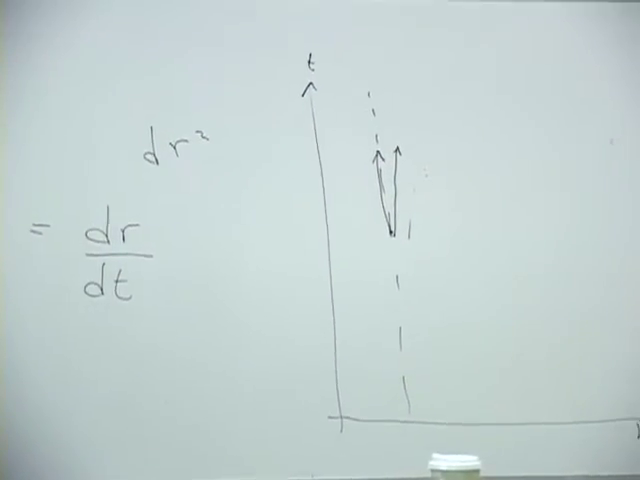
\includegraphics[width=0.82\textwidth]{lecture_02_figure_03.png}
\caption{完成的\(t\)-\(r\)黑板草图：当接近虚线视界时，径向零测地线变得几乎竖直。}
\lectureframe{00:30:25.000}
\end{figure}

\begin{figure}[htbp]
\centering
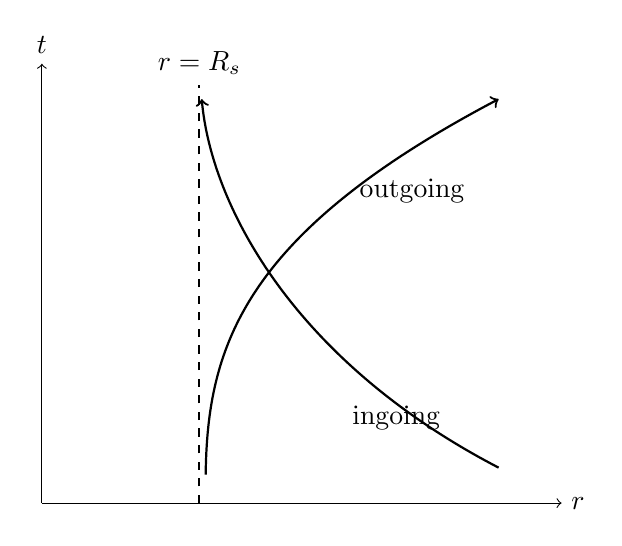
\begin{tikzpicture}[x=1.0cm,y=0.9cm]
\draw[->] (0,0) -- (6.6,0) node[right] {$r$};
\draw[->] (0,0) -- (0,6.2) node[above] {$t$};
\draw[dashed,thick] (2.0,0) -- (2.0,5.9) node[above] {$r=R_s$};
\draw[thick,->] (2.08,.4) .. controls (2.10,2.2) and (2.55,3.8) .. (5.8,5.7);
\draw[thick,->] (5.8,.5) .. controls (3.2,2.0) and (2.15,4.2) .. (2.03,5.7);
\node[align=center] at (4.7,4.4) {outgoing};
\node[align=center] at (4.5,1.2) {ingoing};
\end{tikzpicture}
\caption{黑板草图的坐标时间清理版本。表观减慢是关于Schwarzschild \(t\)的陈述，而不是关于光在局部未能以\(c\)运动的陈述。}
\end{figure}

在视界内部，未来光锥向内倾斜得如此厉害，以至于两个指向未来的径向分支都通向\(r\)减小的方向。任何源自那里的信号都无法逃逸到外部，而每一条指向未来的因果路径都到达奇点。

\begin{classroomqa}
\audiencequestion{如果光速是不变的，那么说光在视界附近减慢究竟是什么意思？\lecturetimestamp{00:31:44}}
\lecturerresponse{所展示的量是在特定坐标系中的\(dr/dt\)。当米被厘米取代时，数值速度就已经改变；在这里，有效的径向和时间标定随位置而变化。普遍的陈述是，每一条光线都遵循零测地线轨迹，\(ds^2=0\)。}
\end{classroomqa}
\editorialnote{自由下落的局部观测者测得真空中的光速为\(c\)；视界处Schwarzschild坐标速度的消失并不是局部可观测量。}

\begin{classroomqa}
\audiencequestion{无论光通过何种物质介质传播，同样的零速度陈述都成立吗？\lecturetimestamp{00:33:24}}
\lecturerresponse{不。现有的认识不再保留对此答案的解释。}
\end{classroomqa}
\editorialnote{零速度论断涉及真空时空中的传播。与物质的相互作用可以使波包具有较小的有效速度；那是介质的性质，而不是局部因果速度\(c\)的改变。}

\begin{classroomqa}
\audiencequestion{在同一個\(t\)-\(r\)图上，入射光线看起来是什么样子？\lecturetimestamp{00:33:32}}
\lecturerresponse{它是看起来反向的分支：从大的\(r\)出发，它向视界弯曲并渐近地接近它。它需要无限多的坐标时间\(t\)才能到达。}
\end{classroomqa}
\editorialnote{下落的观测者在有限的固有时内到达并穿过视界；只有Schwarzschild \(t\)发散。}

\section{为什么蒸发会产生问题}

视界值得更多的研究：它如何形成，下落的观测者看到什么，以及那里是否发生任何局部异常的事情。Susskind推迟了这些问题，直接跳到量子力学。从外部看，物质及其所有可区分的信息被挤压得越来越靠近视界，变得不可获取。仅此一点未必会摧毁信息；它可能只是将其隐藏起来。

Hawking的结果使问题变得尖锐。一个稳定的经典黑洞看起来像可以想象的最乏味的物体：球形、黑暗、无法发送信息。但``黑''有两种含义。它可以意味着不发射任何东西，也可以意味着发射热黑体辐射。量子黑洞是在第二种意义上黑的。它有温度，会发光，并损失能量。由于
\begin{equation}
E=Mc^2,
\qquad
R_s=\frac{2GM}{c^2},
\end{equation}
辐射会同时减小其质量和视界半径。如果蒸发最终移除了黑洞，那么似乎留在其视界处的信息会变成什么？它可能被摧毁，被困在微小的遗迹中，或被编码在出射辐射中。这些可能性之间的张力就是信息问题，而弦理论后来将有助于使它的解决变得更加清晰。

今晚不尝试对弯曲时空中的量子场进行计算。相反，Susskind遵循Bekenstein更简单的路线：首先将熵理解为信息，然后计算黑洞能隐藏多少信息。

\section{存在但被隐藏的信息}

设想把一个盒子划分成足够小的格子，使得每个格子要么被占据，要么为空。每个格子对应一个答案的二进制串---one answer per cell---把该位形与所有其他允许的位形区分开来。更现实的物质需要对粒子种类和其他自由度提出问题，但原理不变：信息由指定状态所需的最少是--否问题数来衡量。

\begin{classroomqa}
\audiencequestion{这只是对一个静态系统的描述吗？\lecturetimestamp{00:45:49}}
\lecturerresponse{这是瞬时的描述，即在一个时刻。动力学随后把该状态映射到另一个状态。}
\end{classroomqa}

下一个原理更为深刻：闭合系统的演化不会把两个不同的微观状态合并为一个。如果两个位形现在不同，它们演化后的位形在原则上仍可区分。经典哈密顿演化是可逆的，量子演化是幺正的。\editorialnote{耗散型有效方程之所以能抹去区别，只是因为未被观测的环境自由度被省略了；完整的闭合状态仍保留它们。}

浴缸把损失与不可及之间的区别具体化。两股水滴流可以编码两段不同的摩尔斯电码文本。水静下来之后，两个浴缸看起来一样。可见的涟漪已经消失，但完整的微观测量仍会发现不同的分子位形。信息已经扩散到太小、太多而无法追踪的自由度中。

熵就是这种隐藏的信息。相对于我们能提出的宏观问题---温度、总能量、成分、水位---许多微观区别仍然可能但不可及。用讲座中数比特的语言，
\begin{equation}
S=\hbox{number of hidden bits}.
\end{equation}
精确的统计公式是\(S=k_B\ln\Omega\)，但定性的定义对黑洞论证已经足够。

\section{温度作为隐藏一个比特的代价}

温度测量起来很熟悉，定义起来却出人意料地间接。Susskind选择熵和能量作为原始概念。假设一个计算机比特被重置到标准值。物理装置仍然存在，但它先前零态和一态之间的区别从计算机中消失了。它不可能从完整世界中消失；它被转移到环境中的微观自由度，使环境轻微升温。这就是Landauer原理。

如果一个熵单位是一个比特，温度以能量单位度量，讲座写出
\begin{align}
\Delta S&=1,\\
\Delta E&=T\,\Delta S,\\
dE&=T\,dS.
\label{eq:first-law}
\end{align}

\begin{figure}[htbp]
\centering
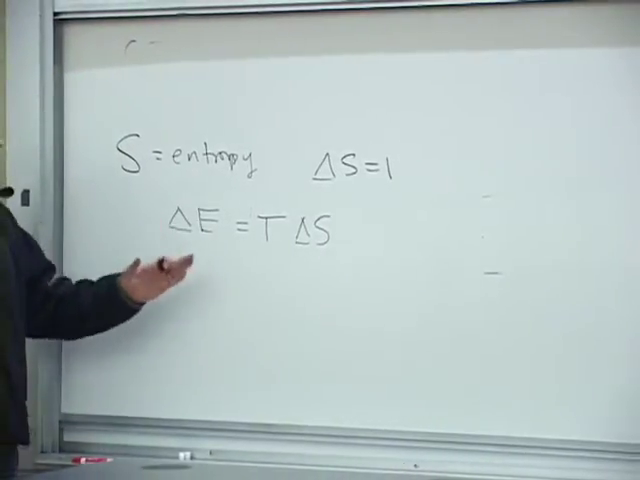
\includegraphics[width=0.84\textwidth]{lecture_02_figure_04.png}
\caption{黑板上的信息论热力学：\(S\)是熵，一个隐藏比特有\(\Delta S=1\)，其最小能量代价写作\(\Delta E=T\Delta S\)。}
\lectureframe{00:58:40.000}
\end{figure}

\editorialnote{在常规单位下，一个二进制比特的可逆擦除代价是\(k_BT\ln2\)。方程~\eqref{eq:first-law}使用\(k_B=1\)，并把讲座的熵单位视为一个比特，同时略去相关的\(\ln2\)。这些约定不影响随后的标度论证。}

听众的估计给出：把大约\(100\)吉字节擦除到一杯水中，引起的最低温升接近\(10^{-15}\)度。Susskind接受这一要点而非确切数字：在室温下，一个比特携带极小的最小能量，而真实计算机耗散得多得多，因为擦除并非可逆地进行。

\begin{classroomqa}
\audiencequestion{硬盘的例子只是类比，还是擦除致热是一条真实的定律？\lecturetimestamp{01:00:02}}
\lecturerresponse{它是一条真实的物理约束，即Landauer规则。重置一个存储单元把旧的区别从计算机中移除，因此该信息必须被带入环境。普通操作的效率远低于理想最小值，因为它们还驱动电路、移动电荷并产生无关的热。}
\end{classroomqa}

\begin{classroomqa}
\audiencequestion{在更高温度下隐藏一个比特要花费更多能量吗？\lecturetimestamp{01:02:07}}
\lecturerresponse{是的。关系\(dE=T\,dS\)正是这样说的：对于相同的熵转移，更热的热浴需要更大的能量转移。人们同样可以把这种每隐藏比特的能量关系视为温度的定义。}
\end{classroomqa}

\begin{classroomqa}
\audiencequestion{如果覆盖一个先前存储的比特，那个旧信息已经丢失了吗？\lecturetimestamp{01:02:43}}
\lecturerresponse{它已经离开计算机，但并未从闭合物理系统中消失。被覆盖的区别已经散布到环境中，在那里它贡献不可及的信息，因而贡献熵。}
\end{classroomqa}

将热力学熵等同于缺失的微观信息，这一思想可追溯到玻尔兹曼；香农在二十世纪给出了与之对应的信息论语言。苏斯金德指出，在他和听众中的一些人在1950年代所接触的热力学课程中，这种解释奇怪地缺席了。计算机科学使这一联系更难被忽视，但并未创造其物理内容。

\section{将一比特放入黑洞}

现在我们可以概念性地逐比特构建一个黑洞，就像浴缸可以逐滴注满一样。问题在于微分层面：当额外一比特被隐藏时，视界增长了多少？从质量为\(M\)、半径为\(R_s\)的黑洞出发，然后送入最简单的物体，其唯一可恢复的区别仅在于是否被吸收。

\begin{classroomqa}
\audiencequestion{信息进入黑洞难道不需要无限坐标时间吗？\lecturetimestamp{01:08:07}}
\lecturerresponse{它在视界附近被指数压缩，在很短的实用时间内对外部不可用，尽管施瓦茨席尔德坐标时间将实际穿越赋予无限值。因此对于外部记账而言，它可以被视为存储在视界上。}
\end{classroomqa}

光子是一个自然的候选者，但一般的光子携带的信息不止一比特。其偏振可以编码一个二元选择。一个高度局域化的到达点提供了许多进一步的是--否问题：上半球还是下半球，左半还是右半，等等。量子力学将局域化限制在约一个波长，因此抑制位置信息的方法是使用黑洞仍能吸收的最长波长。

\begin{classroomqa}
\audiencequestion{真的存在一个光子无法进入的上限波长吗？\lecturetimestamp{01:12:15}}
\lecturerresponse{是的。远大于黑洞的波主要被散射而非吸收。有用的临界选择是波长与视界半径相当：足够长以抹去进入点，又足够短以具有可观的吸收概率。}
\end{classroomqa}

\begin{classroomqa}
\audiencequestion{光子到达的方向本身是否增加了信息？\lecturetimestamp{01:13:28}}
\lecturerresponse{对于与整个视界同量级的波长，场在黑洞上的变化如此缓慢，以至于到达方向无法以精细精度分辨。这就是为什么长波长极限近似为单个是--否数据，而非一个锐利定位的撞击。}
\end{classroomqa}

因此，在量级上选择
\begin{equation}
\lambda\sim R_s=\frac{2GM}{c^2}.
\label{eq:one-bit-wave}
\end{equation}
光子运动学给出
\begin{equation}
E=cp,
\qquad
p=\hbar k=\frac{h}{\lambda},
\qquad
\Delta E\sim\frac{\hbar c}{R_s}.
\label{eq:one-bit-energy}
\end{equation}
这里\(k=2\pi/\lambda\)和\(h=2\pi\hbar\)。讲座刻意忽略了\(2\pi\)，以及量级为一的吸收因子。

\begin{classroomqa}
\audiencequestion{动量应该写成\(\hbar/\lambda\)，还是\(h/\lambda\)？\lecturetimestamp{01:16:00}}
\lecturerresponse{以\(\lambda\)为普通波长时，精确关系是\(p=h/\lambda=2\pi\hbar/\lambda\)；以波数\(k=2\pi/\lambda\)表示时，则是\(p=\hbar k\)。当前的估计只保留量级，因此因子\(2\pi\)被有意舍弃。}
\end{classroomqa}

隐藏一比特的能量代价是温度标度。方程~\eqref{eq:one-bit-wave}和~\eqref{eq:one-bit-energy}因此给出
\begin{equation}
k_BT_H\sim\frac{\hbar c}{R_s}
\sim\frac{\hbar c^3}{GM}.
\end{equation}
精确的霍金结果是
\begin{equation}
k_BT_H=\frac{\hbar c^3}{8\pi GM}.
\end{equation}
基本论证得到了对\(M,G,c,\hbar\)的依赖关系，但未得到系数。

\section{一比特占据一个普朗克尺度斑块}

同一个光子告诉我们视界如何增长。其能量使质量改变
\begin{equation}
\Delta M=\frac{\Delta E}{c^2}
\sim\frac{\hbar}{cR_s}.
\end{equation}
由于\(R_s=2GM/c^2\)，
\begin{equation}
\Delta R_s=\frac{2G}{c^2}\Delta M
\sim\frac{G\hbar}{c^3R_s},
\end{equation}
其中所有量级为一的因子再次被抑制。乘以\(R_s\)，
\begin{equation}
R_s\Delta R_s\sim\frac{G\hbar}{c^3}.
\end{equation}
因为\(A=4\pi R_s^2\)，其微分为\(dA=8\pi R_s\,dR_s\)。因此
\begin{equation}
\Delta A\sim\frac{G\hbar}{c^3}=\ell_P^2,
\qquad
\ell_P=\sqrt{\frac{G\hbar}{c^3}}.
\label{eq:planck-patch}
\end{equation}

\begin{figure}[htbp]
\centering
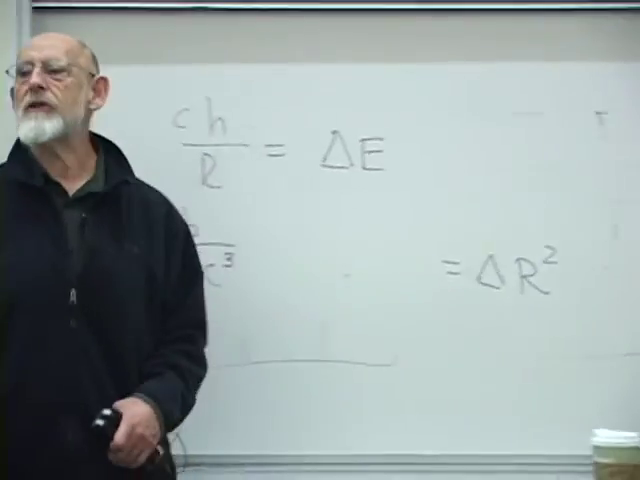
\includegraphics[width=0.84\textwidth]{lecture_02_figure_05.png}
\caption{黑板上完成的标度论证：一比特能量\(\Delta E\sim\hbar c/R_s\)导致半径平方、因而面积的增量约为\(G\hbar/c^3\)。}
\lectureframe{01:22:40.000}
\end{figure}

在现场计算过程中，\(c\)的因子在中途被恢复，一位听众发现了施瓦茨席尔德半径中缺失的\(c^{-2}\)。正是这一修正产生了方程~\eqref{eq:planck-patch}中的\(c^{-3}\)。

\begin{classroomqa}
\audiencequestion{仅在计算的一部分中恢复\(c\)，是否丢失了它的两个幂次？\lecturetimestamp{01:21:18}}
\lecturerresponse{是的。量纲关系是\(R_s=2GM/c^2\)，而非简单的\(2GM\)。恢复该因子使面积标度为\(G\hbar/c^3\)。}
\end{classroomqa}

利用\(G\simeq6.7\times10^{-11}\,\mathrm{m^3\,kg^{-1}\,s^{-2}}\)、\(\hbar\simeq1.05\times10^{-34}\,\mathrm{J\,s}\)和\(c^3\simeq2.7\times10^{25}\,\mathrm{m^3\,s^{-3}}\)，
\begin{equation}
\ell_P^2\simeq2.6\times10^{-70}\,\mathrm{m^2},
\qquad
\ell_P\simeq1.6\times10^{-35}\,\mathrm{m}.
\end{equation}
讲座中口头说出的幂次在黑板上进行估计时有所游移；物理结论是稳定的。这一尺度远低于直接实验分辨率。

令人难忘的图景是：不可穿透的比特带着尖锐的棱角，在视界上堆积，并彼此挤开。每个新比特大约占据一个普朗克面积的斑块。这是对面积记账的一种比喻，并不是说字面意义上的方形瓷砖构成了视界。

\begin{classroomqa}
\audiencequestion{如果第一个光子仍在接近时，另一个光子扩大了视界，那么旧光子难道不会落入新视界之内吗？\lecturetimestamp{01:26:39}}
\lecturerresponse{简单的静态图景不够精确，无法解决这个问题。动态时空中的事件视界必须全局地定义，其位置随着物质到达而改变。在此处所用的外部描述中，信息仍与不断增长的视界相关联。对该视界的精确定义将推迟给出。}
\end{classroomqa}

\begin{classroomqa}
\audiencequestion{当加入巨大质量时，例如两个黑洞碰撞时，会出现同样的问题吗？\lecturetimestamp{01:27:03}}
\lecturerresponse{是的；那时动态特征就无法忽视了。讲座将完整的并合几何推迟到视界被更仔细地定义之后。}
\end{classroomqa}

\begin{classroomqa}
\audiencequestion{普朗克面积是只在平坦斑块上定义的，而不是在球面视界上定义的吗？\lecturetimestamp{01:27:30}}
\lecturerresponse{它是球面上的一个面积尺度，并不要求视界是平坦的。对于这种计数而言，平面与球面的区分并不重要。}
\end{classroomqa}
\editorialnote{当视界曲率半径远大于\(\ell_P\)时，每个普朗克尺度的邻域局部上几乎都是平坦的。}

对于一个直径八公里的黑洞，边缘光子相应地是波长约为该尺度的长射电波。一个面向听众的类比将这种与尺寸无关的面积增量，比作给绕篮球或绕地球的绳子增加相同的额外周长：在每种情况下，由固定增加的周长所产生的径向间隙都相同。精确几何有所不同，但两个例子都分离出了一种与物体原有尺寸无关的变化。

\section{面积定律}

一次增加一个比特，会使视界面积改变一个普适的微观量。因此，能够被隐藏的比特数必须正比于\(A/\ell_P^2\)，而不是正比于体积。贝肯斯坦推断出了这种正比关系；霍金的计算确定了其系数：
\begin{equation}
S_{\mathrm{BH}}=\frac{k_B A c^3}{4G\hbar}
=\frac{k_B A}{4\ell_P^2}.
\label{eq:bh-entropy}
\end{equation}
如果用二进制比特而不是热力学单位来计数熵，则将\(S_{\mathrm{BH}}/k_B\)除以\(\ln2\)。

\begin{figure}[htbp]
\centering
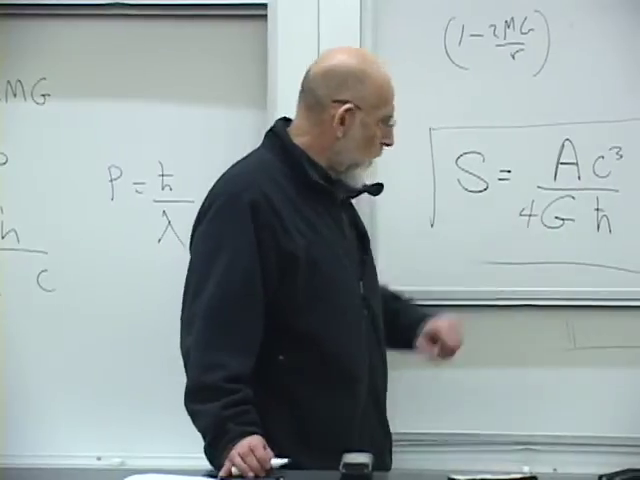
\includegraphics[width=0.84\textwidth]{lecture_02_figure_06.png}
\caption{最终写在黑板上的公式，包括霍金的因子\(1/4\)：在讲座的熵单位中为\(S\propto Ac^3/(4G\hbar)\)。}
\lectureframe{01:31:02.000}
\end{figure}

因此，黑洞比大小相当的普通系统具有更多的熵，而且多出极大的幅度。然而，这个答案仍然小于朴素体积计数可能暗示的结果。独立信息受一个表面测度所界定。这种反转---一个三维的引力区域，由按二维边界标度的信息来描述---正是全息原理的种子。

\begin{classroomqa}
\audiencequestion{熵公式中的因子\(1/4\)从何而来？\lecturetimestamp{01:30:30}}
\lecturerresponse{贝肯斯坦的论证确定了它对面积和基本常数的依赖关系，但留下了一个未知系数；他的估计产生了诸如二的 logarithm 之类的可能性。霍金的量子场计算将该系数精确确定为\(1/4\)。}
\end{classroomqa}

\(\hbar\)的位置包含了最后的惊奇。人们可能期望量子熵正比于\(\hbar\)，并在经典极限下消失。相反，\(\hbar\)出现在分母中。当\(\hbar\to0\)时，波可以以任意小的能量代价携带任意精细的信息，因此熵容量发散。量子化并没有给一个原本经典的洞加上微小的熵；它阻止了信息容量变为无限。

\begin{classroomqa}
\audiencequestion{为什么\(\hbar\)，其单位是角动量，也决定了普通动量与波长之间的关系？\lecturetimestamp{01:33:23}}
\lecturerresponse{\(\hbar\)具有作用量的单位，等价于动量乘以距离。由于\(p\lambda\)具有相同的单位，量子关系可以写成\(p\sim\hbar/\lambda\)，最多相差\(2\pi\)的约定。角动量\(\mathbf r\times\mathbf p\)出于同样的原因具有相同的量纲。}
\end{classroomqa}

讲座到此为止，并非因为主题已经穷尽，而是因为这是一个恰当的边界。几何学已经告诉我们视界为何隐藏信息；热力学已经告诉我们如何计数被隐藏的信息；量子力学则提供了每比特所对应的有限面积。下一个问题不再是黑洞是否具有微观状态，而是这些状态如何编码并最终归还落入其中的东西。
